\documentclass[
  man,
  floatsintext,
  longtable,
  nolmodern,
  notxfonts,
  notimes,
  colorlinks=true,linkcolor=blue,citecolor=blue,urlcolor=blue]{apa7}

\usepackage{amsmath}
\usepackage{amssymb}



\usepackage[bidi=default]{babel}
\babelprovide[main,import]{english}


% get rid of language-specific shorthands (see #6817):
\let\LanguageShortHands\languageshorthands
\def\languageshorthands#1{}

\RequirePackage{longtable}
\RequirePackage{threeparttablex}

\makeatletter
\renewcommand{\paragraph}{\@startsection{paragraph}{4}{\parindent}%
	{0\baselineskip \@plus 0.2ex \@minus 0.2ex}%
	{-.5em}%
	{\normalfont\normalsize\bfseries\typesectitle}}

\renewcommand{\subparagraph}[1]{\@startsection{subparagraph}{5}{0.5em}%
	{0\baselineskip \@plus 0.2ex \@minus 0.2ex}%
	{-\z@\relax}%
	{\normalfont\normalsize\bfseries\itshape\hspace{\parindent}{#1}\textit{\addperi}}{\relax}}
\makeatother




\usepackage{longtable, booktabs, multirow, multicol, colortbl, hhline, caption, array, float, xpatch}
\setcounter{topnumber}{2}
\setcounter{bottomnumber}{2}
\setcounter{totalnumber}{4}
\renewcommand{\topfraction}{0.85}
\renewcommand{\bottomfraction}{0.85}
\renewcommand{\textfraction}{0.15}
\renewcommand{\floatpagefraction}{0.7}

\usepackage{tcolorbox}
\tcbuselibrary{listings,theorems, breakable, skins}
\usepackage{fontawesome5}

\definecolor{quarto-callout-color}{HTML}{909090}
\definecolor{quarto-callout-note-color}{HTML}{0758E5}
\definecolor{quarto-callout-important-color}{HTML}{CC1914}
\definecolor{quarto-callout-warning-color}{HTML}{EB9113}
\definecolor{quarto-callout-tip-color}{HTML}{00A047}
\definecolor{quarto-callout-caution-color}{HTML}{FC5300}
\definecolor{quarto-callout-color-frame}{HTML}{ACACAC}
\definecolor{quarto-callout-note-color-frame}{HTML}{4582EC}
\definecolor{quarto-callout-important-color-frame}{HTML}{D9534F}
\definecolor{quarto-callout-warning-color-frame}{HTML}{F0AD4E}
\definecolor{quarto-callout-tip-color-frame}{HTML}{02B875}
\definecolor{quarto-callout-caution-color-frame}{HTML}{FD7E14}

%\newlength\Oldarrayrulewidth
%\newlength\Oldtabcolsep


\usepackage{hyperref}




\providecommand{\tightlist}{%
  \setlength{\itemsep}{0pt}\setlength{\parskip}{0pt}}
\usepackage{longtable,booktabs,array}
\usepackage{calc} % for calculating minipage widths
% Correct order of tables after \paragraph or \subparagraph
\usepackage{etoolbox}
\makeatletter
\patchcmd\longtable{\par}{\if@noskipsec\mbox{}\fi\par}{}{}
\makeatother
% Allow footnotes in longtable head/foot
\IfFileExists{footnotehyper.sty}{\usepackage{footnotehyper}}{\usepackage{footnote}}
\makesavenoteenv{longtable}

\usepackage{graphicx}
\makeatletter
\def\maxwidth{\ifdim\Gin@nat@width>\linewidth\linewidth\else\Gin@nat@width\fi}
\def\maxheight{\ifdim\Gin@nat@height>\textheight\textheight\else\Gin@nat@height\fi}
\makeatother
% Scale images if necessary, so that they will not overflow the page
% margins by default, and it is still possible to overwrite the defaults
% using explicit options in \includegraphics[width, height, ...]{}
\setkeys{Gin}{width=\maxwidth,height=\maxheight,keepaspectratio}
% Set default figure placement to htbp
\makeatletter
\def\fps@figure{htbp}
\makeatother


% definitions for citeproc citations
\NewDocumentCommand\citeproctext{}{}
\NewDocumentCommand\citeproc{mm}{%
  \begingroup\def\citeproctext{#2}\cite{#1}\endgroup}
\makeatletter
 % allow citations to break across lines
 \let\@cite@ofmt\@firstofone
 % avoid brackets around text for \cite:
 \def\@biblabel#1{}
 \def\@cite#1#2{{#1\if@tempswa , #2\fi}}
\makeatother
\newlength{\cslhangindent}
\setlength{\cslhangindent}{1.5em}
\newlength{\csllabelwidth}
\setlength{\csllabelwidth}{3em}
\newenvironment{CSLReferences}[2] % #1 hanging-indent, #2 entry-spacing
 {\begin{list}{}{%
  \setlength{\itemindent}{0pt}
  \setlength{\leftmargin}{0pt}
  \setlength{\parsep}{0pt}
  % turn on hanging indent if param 1 is 1
  \ifodd #1
   \setlength{\leftmargin}{\cslhangindent}
   \setlength{\itemindent}{-1\cslhangindent}
  \fi
  % set entry spacing
  \setlength{\itemsep}{#2\baselineskip}}}
 {\end{list}}
\usepackage{calc}
\newcommand{\CSLBlock}[1]{\hfill\break\parbox[t]{\linewidth}{\strut\ignorespaces#1\strut}}
\newcommand{\CSLLeftMargin}[1]{\parbox[t]{\csllabelwidth}{\strut#1\strut}}
\newcommand{\CSLRightInline}[1]{\parbox[t]{\linewidth - \csllabelwidth}{\strut#1\strut}}
\newcommand{\CSLIndent}[1]{\hspace{\cslhangindent}#1}





\usepackage{newtx}

\defaultfontfeatures{Scale=MatchLowercase}
\defaultfontfeatures[\rmfamily]{Ligatures=TeX,Scale=1}





\title{The relationship between international study and civic virtues}


\shorttitle{The relationship between international study and civic
virtues}


\usepackage{etoolbox}






\author{Yangyue Li}



\affiliation{
{MA Program in the Social Sciences, University of Chicago}}




\leftheader{Li}



\abstract{This study investigated civic virtues among international and
American undergraduate students to examine potential differences in
psychological constructs associated with civic development. we compared
86 students from a single university across multiple measures of civic
virtues, including relational civility, civic attitudes and behaviors,
empathy, epistemic humility, and cultural competence. Independent
samples t-tests and one-way analyses of variance found no statistically
significant differences between international and American students
across these constructs. The findings suggest that the contemporary
university experience may promote comparable civic development
trajectories, regardless of students' international status.}

\keywords{civic virtues, empathy, wisdom, civility, international
studies}

\authornote{ 

\par{       }
\par{Correspondence concerning this article should be addressed
to Yangyue Li, MA Program in the Social Sciences, University of
Chicago, 1155 E 60th
St., Chicago, IL 60637, USA, Email: yangyueli28@uchicago.edu}
}

\makeatletter
\let\endoldlt\endlongtable
\def\endlongtable{
\hline
\endoldlt
}
\makeatother

\urlstyle{same}



\usepackage{booktabs}
\usepackage{longtable}
\usepackage{array}
\usepackage{multirow}
\usepackage{wrapfig}
\usepackage{float}
\usepackage{colortbl}
\usepackage{pdflscape}
\usepackage{tabu}
\usepackage{threeparttable}
\usepackage{threeparttablex}
\usepackage[normalem]{ulem}
\usepackage{makecell}
\usepackage{xcolor}
\makeatletter
\@ifpackageloaded{caption}{}{\usepackage{caption}}
\AtBeginDocument{%
\ifdefined\contentsname
  \renewcommand*\contentsname{Table of contents}
\else
  \newcommand\contentsname{Table of contents}
\fi
\ifdefined\listfigurename
  \renewcommand*\listfigurename{List of Figures}
\else
  \newcommand\listfigurename{List of Figures}
\fi
\ifdefined\listtablename
  \renewcommand*\listtablename{List of Tables}
\else
  \newcommand\listtablename{List of Tables}
\fi
\ifdefined\figurename
  \renewcommand*\figurename{Figure}
\else
  \newcommand\figurename{Figure}
\fi
\ifdefined\tablename
  \renewcommand*\tablename{Table}
\else
  \newcommand\tablename{Table}
\fi
}
\@ifpackageloaded{float}{}{\usepackage{float}}
\floatstyle{ruled}
\@ifundefined{c@chapter}{\newfloat{codelisting}{h}{lop}}{\newfloat{codelisting}{h}{lop}[chapter]}
\floatname{codelisting}{Listing}
\newcommand*\listoflistings{\listof{codelisting}{List of Listings}}
\makeatother
\makeatletter
\makeatother
\makeatletter
\@ifpackageloaded{caption}{}{\usepackage{caption}}
\@ifpackageloaded{subcaption}{}{\usepackage{subcaption}}
\makeatother

% From https://tex.stackexchange.com/a/645996/211326
%%% apa7 doesn't want to add appendix section titles in the toc
%%% let's make it do it
\makeatletter
\xpatchcmd{\appendix}
  {\par}
  {\addcontentsline{toc}{section}{\@currentlabelname}\par}
  {}{}
\makeatother

%% Disable longtable counter
%% https://tex.stackexchange.com/a/248395/211326

\usepackage{etoolbox}

\makeatletter
\patchcmd{\LT@caption}
  {\bgroup}
  {\bgroup\global\LTpatch@captiontrue}
  {}{}
\patchcmd{\longtable}
  {\par}
  {\par\global\LTpatch@captionfalse}
  {}{}
\apptocmd{\endlongtable}
  {\ifLTpatch@caption\else\addtocounter{table}{-1}\fi}
  {}{}
\newif\ifLTpatch@caption
\makeatother

\begin{document}

\maketitle


\setcounter{secnumdepth}{-\maxdimen} % remove section numbering

\setlength\LTleft{0pt}


In an interconnected world, civic virtues are crucial for fostering
responsible citizenship and encouraging individuals to prioritize
societal well-being over self-interest
(\citeproc{ref-sherrodDimensionsCitizenshipOpportunities2002}{Sherrod et
al., 2002}). U.S. universities, as diverse microcosms, bring domestic
and international students together, offering unique contexts for civic
engagement and understanding the values of others. Domestic American
students may develop civic engagement through strong ties to their local
communities and the American education system, while international
students may bring perspectives shaped by cross-cultural experiences and
adaptation to a new cultural environment. Undergoing the same admission
process and sharing similar college life on campus with their American
peers, international students may still differ in civic behaviors. These
contexts raise critical questions about the factors that foster civic
virtues and motivate individuals to engage in civic-minded behaviors.
How do experiences in a foreign and culturally different environment
influence civic virtues and related psychological characteristics such
as empathy and cultural competence? Do international students differ on
these psychological aspects from US students?

\subsection{Literature Review}\label{literature-review}

\subsubsection{Education and Civic
Virtues}\label{education-and-civic-virtues}

Civic engagement may foster a sense of belonging, purpose, and
responsibility within a community, and may empower individuals to
contribute to a common good
(\citeproc{ref-flanaganCivicEngagementTransition2010}{Flanagan \&
Levine, 2010}). Research suggests that civic education - educational
experiences that are directed at increasing civic virtues - happens
mostly during adolescence, but can continue into young adulthood
(\citeproc{ref-flanaganCivicEngagementTransition2010}{Flanagan \&
Levine, 2010};
\citeproc{ref-sherrodDimensionsCitizenshipOpportunities2002}{Sherrod et
al., 2002}). Much of this experience occurs in educational settings,
particularly colleges, which offer structured opportunities through
coursework, extracurricular activities, community service programs, and
student organizations
(\citeproc{ref-flanaganCivicEngagementTransition2010}{Flanagan \&
Levine, 2010}). These experiences could help young adults develop civic
virtues and social responsibility.

Besides formal instruction in character education and civility
(\citeproc{ref-jeynesMetaAnalysisRelationshipCharacter2019}{Jeynes,
2019};
\citeproc{ref-torney-purtaSchoolsRoleDeveloping2002}{Torney-Purta,
2002}), non-didactic and informal experiences have important
implications for the development of civic virtues as well. Indeed,
research highlights that youths who are involved in community-based
organizations or extracurricular activities are more likely to be
civically active
(\citeproc{ref-zarrettRoleOrganizedActivities2021}{Zarrett et al.,
2021}). Furthermore, a study suggests that participating in community
service or volunteering is associated with adolescent civic beliefs
about considering similar types of civic engagement behaviors
(\citeproc{ref-metzgerAdolescentsCivicEngagement2019}{Metzger et al.,
2019}). Similarly, Vézina and Poulin
(\citeproc{ref-vezinaInvestigatingCivicParticipation2019}{2019}) found
that prosocial/community-based activities are related to a greater
likelihood of being in the high-sustained civic engagement trajectory.

Additionally, recent research suggests that study abroad programs may
increase some aspects of civic virtues and related psychological
capacities. Living and studying in a foreign cultural environment
provide opportunities for students to interact with people from diverse
backgrounds, fostering skills related to civic virtues such as empathy,
open-mindedness, and perspective-taking in a non-didactic way
(\citeproc{ref-chieffoLargeScaleAssessmentStudent2004}{Chieffo \&
Griffiths, 2004}). Research indicates that even short-term study abroad
programs enhance student's empathy and open-mindedness toward diverse
perspectives, and foster a deeper sense of responsibility as global
citizens (\citeproc{ref-chieffoLargeScaleAssessmentStudent2004}{Chieffo
\& Griffiths, 2004}). Black and Duhon
(\citeproc{ref-blackAssessingImpactBusiness2006}{2006}) assessed the
impact of a month-long business-focused study abroad program in London
on students' cultural awareness and personal development. Consistent
with previous findings, students showed significant improvements in
cross-cultural empathy and understanding of global perspectives. A more
recent study examined the relationship between studying abroad and civic
virtues (\citeproc{ref-boulwareStrangerStrangeLand2023}{Boulware et al.,
2023}). The results suggest that undergraduate students who have gone
abroad via one particular set of study abroad programs in undergraduate
studies demonstrated higher levels of empathy, civic engagement, and
civility toward others, compared with students who do not have these
experiences or have no interest in them.

\subsubsection{International Students and Civic
Virtues}\label{international-students-and-civic-virtues}

Universities in the United States enroll a substantial number of
international students annually, yet the benefits for this population
remain underexplored in respect of non-curricular benefits. Research on
a variety of different psychological capacities wisdom, bilingualism,
and cultural adaptation may offer insights into the interaction of
personal and contextual factors that could shape civic virtues among
international students. As Staudinger et al.
(\citeproc{ref-staudingerWhatPredictsWisdomrelated1998}{1998}) point
out, virtues are a fundamental component of wisdom, with openness to
experience and social competence serving as critical predictors of
wisdom-related performance
(\citeproc{ref-baltesFascinationWisdomIts2008}{Baltes \& Smith, 2008}).
Similarly, (\citeproc{ref-grossmannWisdomContext2017}{Grossmann, 2017})
illustrates how contextual factors, such as cultural and experiential
environments, shape wisdom-related reasoning and behaviors.
International students, who frequently navigate diverse cultural and
educational settings, may adapt their civic engagement to align with
situational demands.

\subsubsection{Current Study}\label{current-study}

Although international students represent a substantial portion of the
US college population and can play an important role in civic life,
there is little research on how this experience relates to civic
virtues. This study aims to investigate civic virtues among
international students studying in the United States. The primary goals
are to answer the key research question: do international students, due
to their unique experiences in a foreign country, exhibit similar or
differing levels of civic virtues compared to American students? Given
that study abroad experiences can positively influence one's civility,
we hypothesize that international students may exhibit higher levels of
civic virtues than American students with no experience studying abroad.
This would be comparable to US students who study abroad suggesting that
living in a foreign country may be an important experience related to
civic virtues. Alternatively, international students may score higher on
some psychological characteristics related to civic virtue development,
including epistemic humility, empathy, need for cognition (NFC), and
cultural competence, while showing comparable levels of civic attitudes
and behaviors.

\section{Method}\label{method}

\subsection{Participants}\label{participants}

\begin{table}

{\caption{{Demographic Characteristics of
Participants}{\label{tbl-demographics}}}
\vspace{-20pt}}

\begin{longtable*}[t]{llll}
\toprule
Label & Level & American & International\\
\midrule
Age (years) & Mean (SD) & 19.39 (0.89) & 19.77 (1.10)\\
Gender & Female & 38 (67.9\%) & 14 (46.7\%)\\
 & Male & 17 (30.4\%) & 14 (46.7\%)\\
 & Prefer not to answer & 1 (1.8\%) & 2 (6.7\%)\\
Ethnicity & Asian & 21 (37.5\%) & 18 (60.0\%)\\
\addlinespace
 & Black or African American & 5 (8.9\%) & NA\\
 & Not specified & 1 (1.8\%) & NA\\
 & Prefer not to answer & 2 (3.6\%) & 2 (6.7\%)\\
 & Prefer to self-describe & 2 (3.6\%) & 2 (6.7\%)\\
 & Two or more races & 6 (10.7\%) & 1 (3.3\%)\\
\addlinespace
 & White & 18 (32.1\%) & 7 (23.3\%)\\
 & NA & 1 (1.8\%) & NA\\
\bottomrule
\end{longtable*}

\end{table}

A survey was adapted from Boulware et al.~(2023). Participants were
recruited through the Psychology Department's SONA system during the
winter quarter in 2025 as well as through campus advertisements. The
total sample consisted of 86 participants, with 30 international
students and 56 domestic students, representing a diverse composition of
student backgrounds as detailed in Table~\ref{tbl-demographics}.

\subsection{Measures}\label{measures}

A survey was adapted from Boulware et al.~(2023), and distributed
through the Psychology Department's research participant recruitment
system during the winter quarter in 2025.

\subsubsection{Civic Virtues}\label{civic-virtues}

We will use two measures to assess civic virtues. The first is Doolittle
and Faul's (2013) 14-item Civic Engagement Scale. It includes the 8
civic attitude subscale (e.g., ``I feel responsible for my community'',
1 = disagree, and 7 = agree) and 6 civic behavior items (e.g., ``I am
involved in structured volunteer position(s) in the community'', 1 =
never, and 7 = always). The second one is based on the Workplace
Relational Civility scale, tailored for student population. It includes
13 items assessing civility towards others and 13 items assessing
civility experienced by participants (Di Fabio \& Gori, 2016). Sample
items include ``I was able to express my values and my beliefs calmly to
others'' and ``Others were able to express their point of view without
being disrespectful toward me'' (1= not at all, and 5 = a great deal).

\subsubsection{Other constructs related to civic
virtues}\label{other-constructs-related-to-civic-virtues}

We will use a scale developed at the Center for Practical Wisdom at the
University of Chicago to assess epistemic humility (Hoeckner, 2011,
personal communication). Sample items include ``I accept that many good
and bad things happening to me are beyond my control'' (1 = strongly
disagree, and 8 = strongly agree). We will use the 8-item Empathy
Quotient to measure empathy towards others
(\citeproc{ref-loewenEightitemFormEmpathy}{Loewen et al., n.d.}). Sample
items include ``I find it easy to put myself in somebody else's shoes''
(1 = never, and 5 = always). We will use the 6-item NFC short form scale
to measure the tendency to engage in cognitive effort
(\citeproc{ref-linsdeholandacoelhoVeryEfficientAssessment2020}{Lins De
Holanda Coelho et al., 2020}). Sample questions include ``I would prefer
complex to simple problems'' (1 = extremely uncharacteristic, and 5 =
extremely characteristic). We will measure cultural competency based on
a set of questions provided by the Study Abroad program at the
University of Chicago. For international students, we will have
questions asking them to report their first language, English
proficiency (indicated by the Test of English as a Foreign Language or a
self-report scale), and duration of their residence in the United
States. American students will indicate whether they have studied
abroad.

\subsection{Data Analysis}\label{data-analysis}

To test the first hypothesis, independent t-tests compared international
and American students on each measure of civic virtues (civic attitudes,
civic behaviors, and civility) and other related constructs. These
comparisons indicated whether international students, as a group,
exhibit different levels of civic virtues compared to their American
peers. An Analysis of Variance (ANOVA) will be conducted to account for
relationships among the dependent variables and provide a more
comprehensive analysis.

\section{Results}\label{results}

\subsection{Descriptive Analyses}\label{descriptive-analyses}

\begin{table}

{\caption{{Descriptive Statistics of Civic Virtues
Measures}{\label{tbl-descriptive-stats}}}
\vspace{-20pt}}

\begin{tabular}[t]{lrrrrr}
\toprule
Variable & Mean & SD & Median & Min & Max\\
\midrule
CB\_CA Total & 72.05 & 14.34 & 72.0 & 33 & 98\\
Civic Attitudes & 43.52 & 8.51 & 43.0 & 20 & 56\\
Civic Behaviors & 28.52 & 7.18 & 28.5 & 13 & 42\\
Civility Total & 101.81 & 13.36 & 101.5 & 73 & 130\\
Civility Towards Me & 48.30 & 8.57 & 48.5 & 28 & 65\\
\addlinespace
Civility Towards Others & 53.51 & 6.86 & 53.0 & 36 & 65\\
Cultural Competence & 34.16 & 4.39 & 34.5 & 19 & 43\\
Empathy & 29.41 & 3.65 & 30.0 & 22 & 37\\
Epistemic Humility & 94.52 & 12.88 & 95.5 & 62 & 122\\
Need for Closure & 57.88 & 12.35 & 57.0 & 30 & 91\\
\addlinespace
Need for Cognition & 21.71 & 3.87 & 22.0 & 12 & 30\\
Wise Reasoning & 76.59 & 12.81 & 76.5 & 26 & 105\\
\bottomrule
\end{tabular}

\end{table}

Descriptive statistics for the key measures of civic virtues are
presented in Table~\ref{tbl-descriptive-stats}. The sample exhibited
varying levels of psychological constructs related to civic engagement.
\emph{Civic Attitudes} showed a mean of 43.52 (\emph{SD} = 8.51), with a
range from 20 to 56. \emph{Civic Behaviors} displayed a mean of 28.52
(\emph{SD} = 7.18), suggesting moderate levels of community engagement.

The variability across different civic virtue measures suggests
potential differences in how participants conceptualize and enact civic
engagement. \emph{Epistemic Humility}, for instance, ranged from 62 to
122, with a mean of 94.52 (\emph{SD} = 12.88), indicating considerable
individual variation in this construct.

\subsection{Bivariate Correlations}\label{bivariate-correlations}

\begin{table}

{\caption{{Bivariate Correlations among Civic Virtues
Constructs}{\label{tbl-correlations}}}
\vspace{-20pt}}

[!h]
\centering
\resizebox{\ifdim\width>\linewidth\linewidth\else\width\fi}{!}{
\begin{tabular}[t]{lllllllll}
\toprule
Variable & Civility Total & CB\_CA Total & Wise Reasoning & Need for Cognition & Empathy & Need for Closure & Epistemic Humility & Cultural Competence\\
\midrule
Civility Total & 1.000 & 0.433*** & 0.377*** & 0.215* & 0.272* & 0.014ns & 0.394*** & 0.294**\\
CB\_CA Total & 0.433*** & 1.000 & 0.273* & 0.359** & 0.05ns & 0.195ns & 0.404*** & 0.272*\\
Wise Reasoning & 0.377*** & 0.273* & 1.000 & 0.128ns & 0.146ns & -0.042ns & 0.239* & 0.24*\\
Need for Cognition & 0.215* & 0.359** & 0.128ns & 1.000 & 0.089ns & -0.075ns & 0.161ns & 0.32**\\
Empathy & 0.272* & 0.05ns & 0.146ns & 0.089ns & 1.000 & -0.367** & 0.093ns & 0.416***\\
\addlinespace
Need for Closure & 0.014ns & 0.195ns & -0.042ns & -0.075ns & -0.367** & 1.000 & -0.048ns & -0.215*\\
Epistemic Humility & 0.394*** & 0.404*** & 0.239* & 0.161ns & 0.093ns & -0.048ns & 1.000 & 0.34**\\
Cultural Competence & 0.294** & 0.272* & 0.24* & 0.32** & 0.416*** & -0.215* & 0.34** & 1.000\\
\bottomrule
\end{tabular}}

\end{table}

\begin{figure}

\caption{\label{fig-correlation-plot}Correlation Matrix of Civic Virtues
Constructs}

\centering{

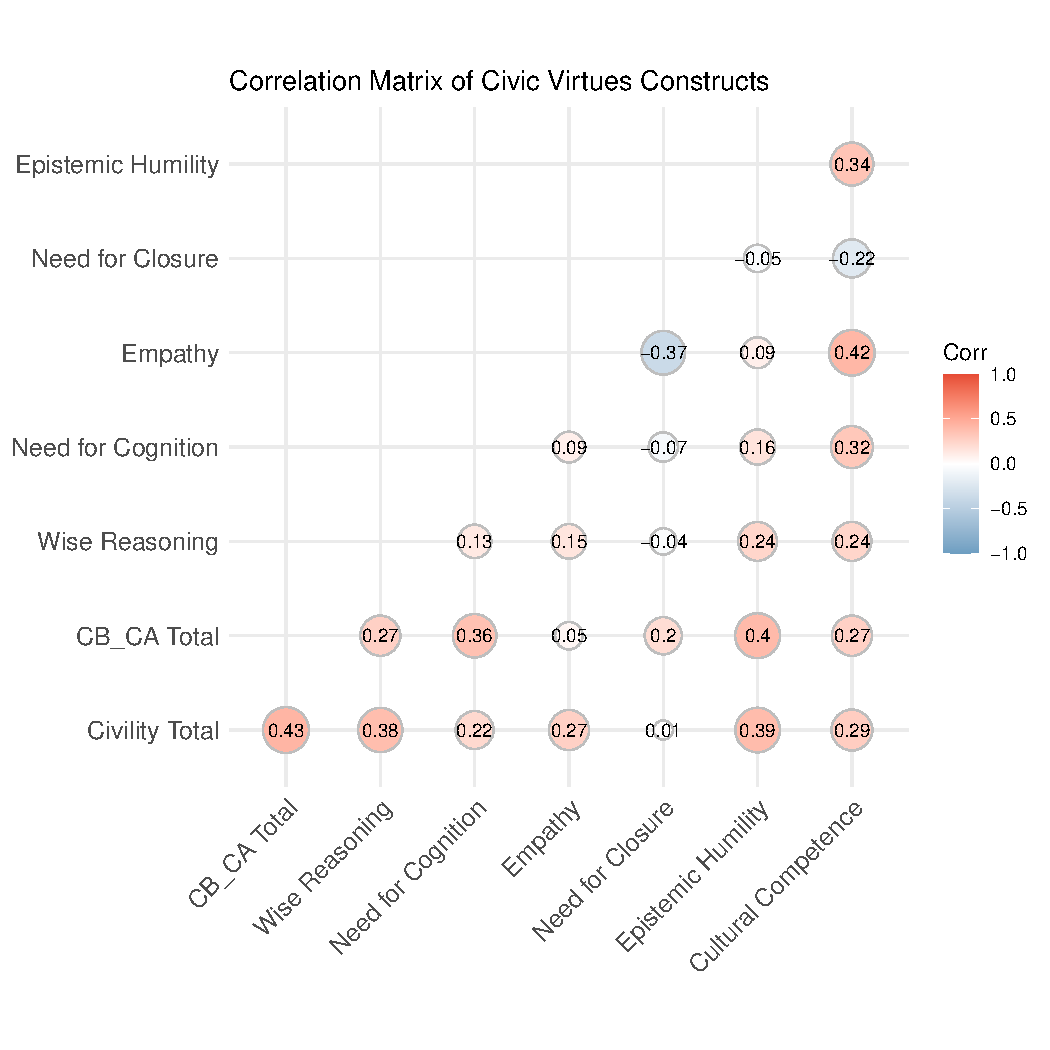
\includegraphics{civic-virtues-yyli28_files/figure-pdf/fig-correlation-plot-1.pdf}

}

\end{figure}%

The correlation matrix presented in Table~\ref{tbl-correlations} and
visualized in Figure~\ref{fig-correlation-plot} provides a comprehensive
view of these intricate relationships. \emph{CB\_CA Total} was
moderately correlated with \emph{Wise Reasoning} (r = 0.273, p = 0.011),
suggesting an interconnection between behavioral and cognitive aspects
of civic engagement. \emph{Empathy} showed notable correlations with
several constructs. It was moderately correlated with \emph{Wise
Reasoning} (r = 0.146, p = 0.181), and significantly associated with
\emph{Epistemic Humility} (r = 0.093, p = 0.393). These relationships
highlight the potential interconnectedness of psychological
characteristics related to civic virtues. \emph{Cultural Competence}
demonstrated interesting associations, including a moderate correlation
with \emph{Need for Cognition} (r = 0.32, p = 0.003). The significant
correlations, marked with asterisks in Table~\ref{tbl-correlations},
indicate the complex interplay between different psychological
constructs related to civic engagement.\footnote{Significance levels are
  indicated as follows: \emph{p} \textless{} 0.05, \textbf{p}
  \textless{} 0.01, \textbf{\emph{p}} \textless{} 0.001.}

\subsection{T-tests}\label{t-tests}

\begin{table}

{\caption{{Comparison of Civic Virtues Constructs between American and
International Students}{\label{tbl-t-tests}}}
\vspace{-20pt}}

[!h]
\centering
\resizebox{\ifdim\width>\linewidth\linewidth\else\width\fi}{!}{
\begin{tabular}[t]{lrrrrrrr}
\toprule
Variable & t & df & p & M (American) & SD (American) & M (International) & SD (International)\\
\midrule
Civility Total & -0.060 & 84 & 0.952 & 101.750 & 12.457 & 101.933 & 15.131\\
CB\_CA Total & 0.794 & 84 & 0.430 & 72.946 & 14.916 & 70.367 & 13.265\\
Wise Reasoning & -0.285 & 84 & 0.777 & 76.304 & 13.622 & 77.133 & 11.349\\
Need for Cognition & 0.133 & 84 & 0.895 & 21.750 & 3.684 & 21.633 & 4.255\\
Empathy & 0.943 & 84 & 0.348 & 29.679 & 3.454 & 28.900 & 3.994\\
\addlinespace
Need for Closure & 0.703 & 84 & 0.484 & 58.571 & 12.823 & 56.600 & 11.530\\
Epistemic Humility & 0.257 & 84 & 0.798 & 94.786 & 12.036 & 94.033 & 14.521\\
Cultural Competence & 0.610 & 84 & 0.544 & 34.375 & 3.840 & 33.767 & 5.328\\
\bottomrule
\end{tabular}}

\end{table}

\begin{figure}

\caption{\label{fig-t-test-viz}Comparison of Civic Virtues Constructs
between American and International Students}

\centering{

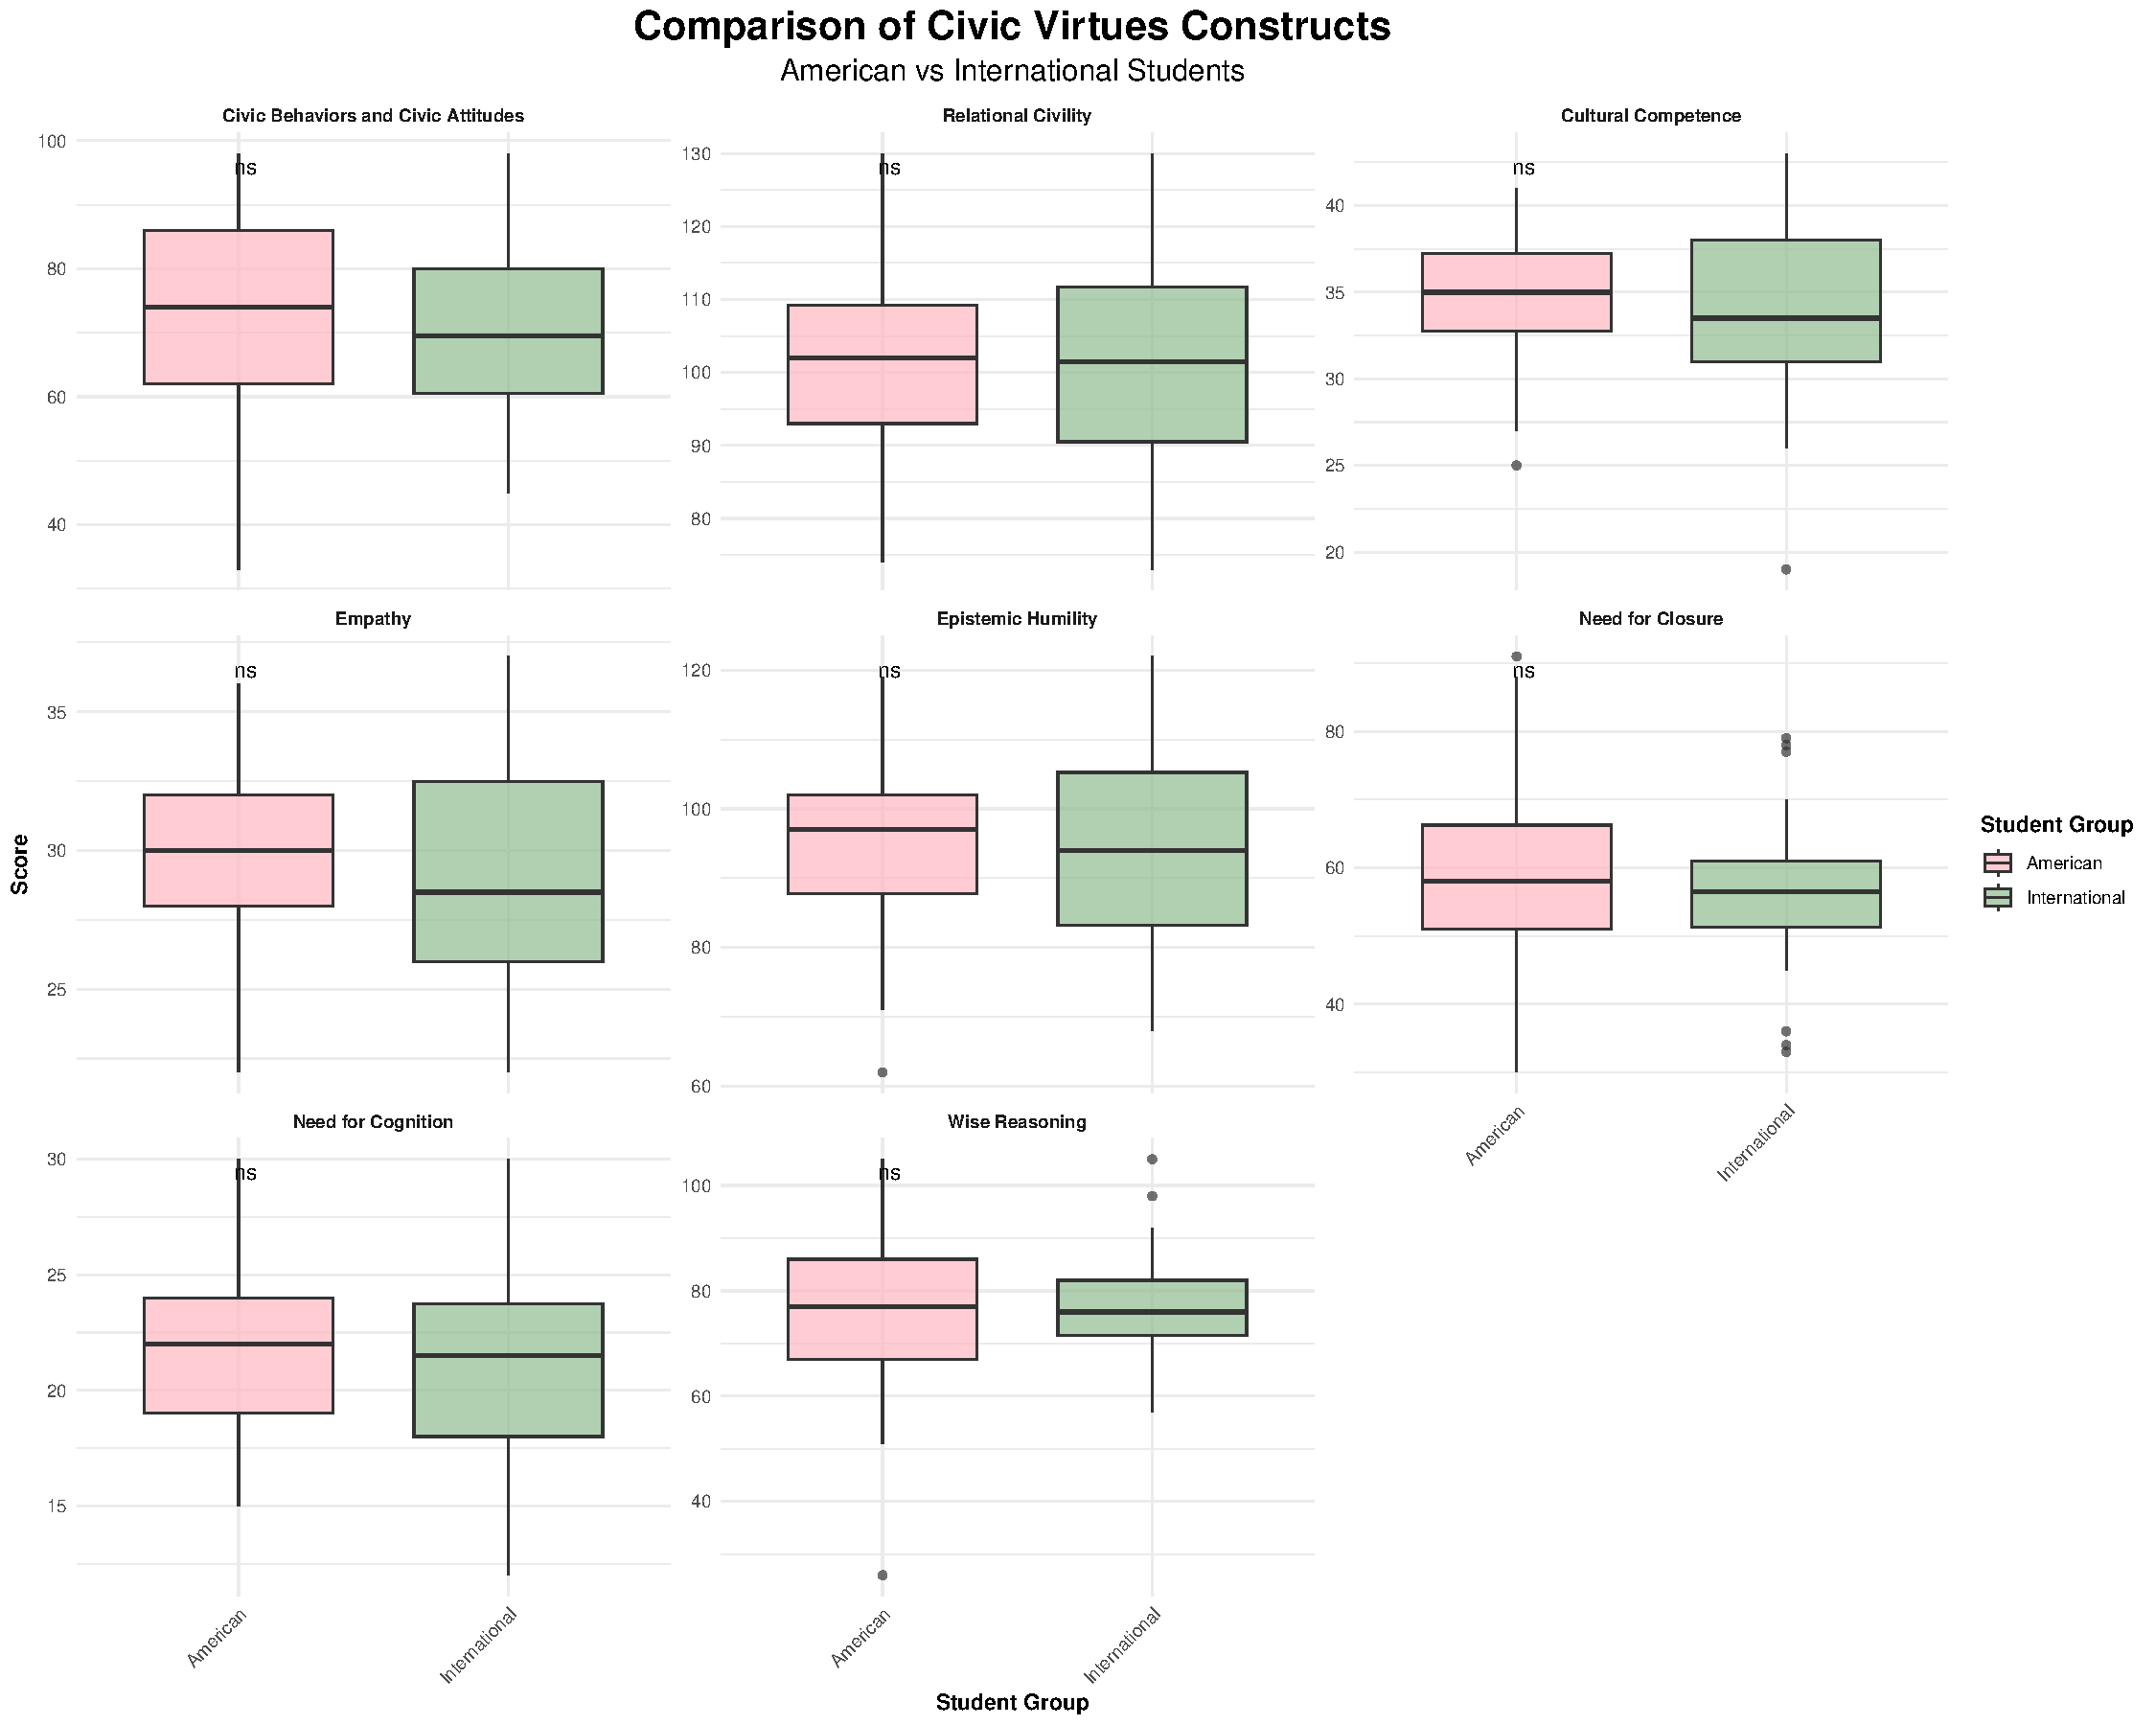
\includegraphics{civic-virtues-yyli28_files/figure-pdf/fig-t-test-viz-1.pdf}

}

\end{figure}%

\begin{figure}

\caption{\label{fig-civic-behaviors-attitudes}Differences in Civic
Behaviors and Civic Attitudes Between International and American
Students}

\centering{

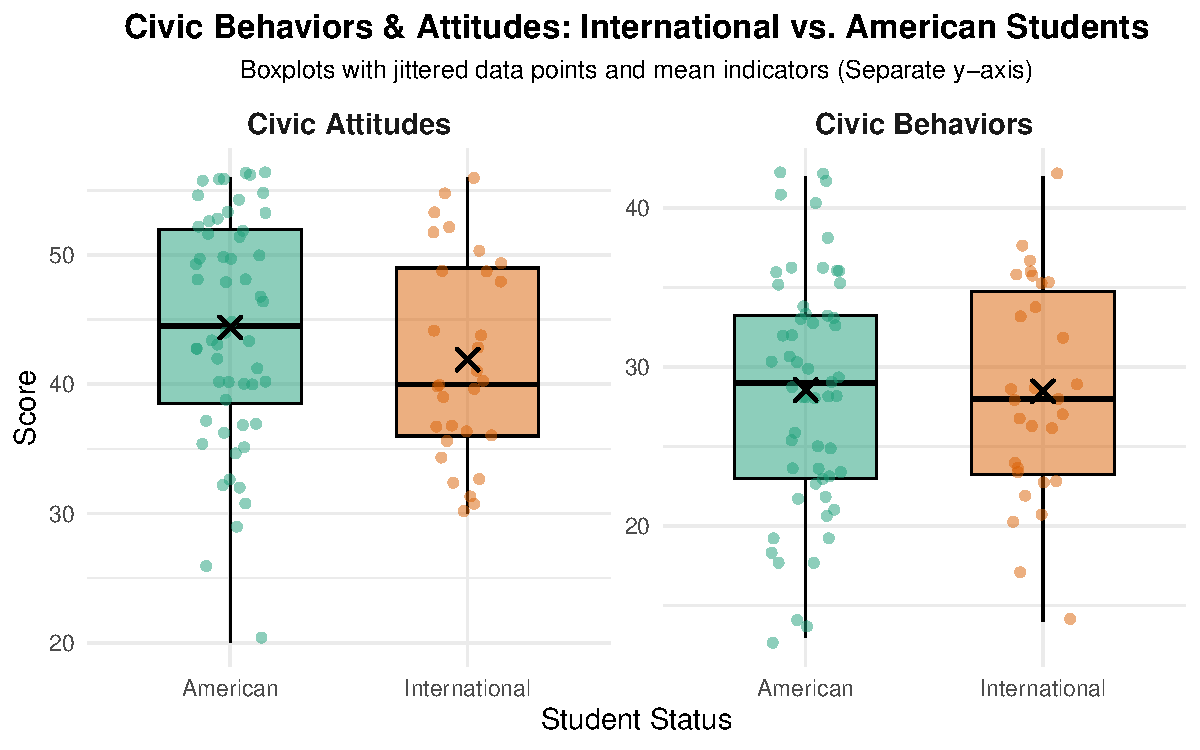
\includegraphics{civic-virtues-yyli28_files/figure-pdf/fig-civic-behaviors-attitudes-1.pdf}

}

\end{figure}%

\begin{figure}

\caption{\label{fig-civility-me-others}Differences in Civility Towards
Me and Civility Towards Others Between International and American
Students}

\centering{

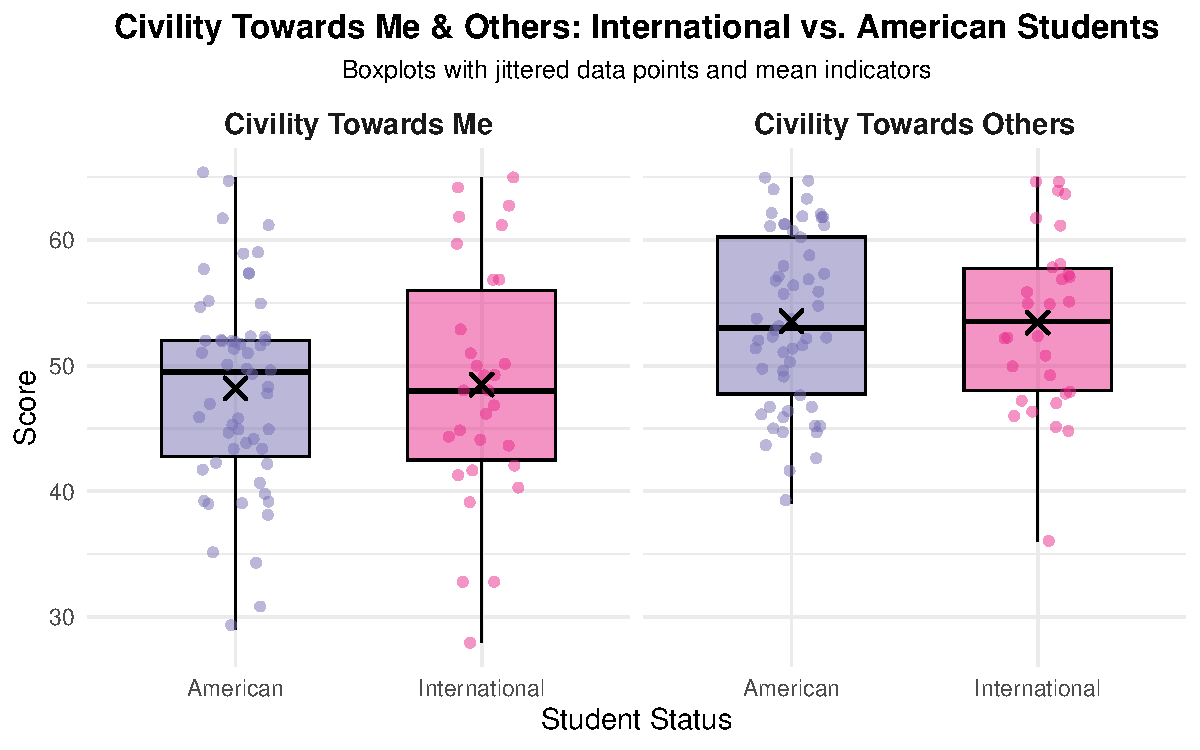
\includegraphics{civic-virtues-yyli28_files/figure-pdf/fig-civility-me-others-1.pdf}

}

\end{figure}%

The dataset includes a total of 3 student groups. However, in this
study, we only compared American students with international students.
To examine differences between American students (including those with
study abroad experience) and international students, a series of
independent samples t-tests were conducted across key civic and civility
constructs. The results are summarized in Table~\ref{tbl-t-tests} and
Figure~\ref{fig-t-test-viz}. No siginificant differences were found in
all of these constructs. An independent samples t-test was conducted to
examine differences in Civic Attitudes (CA) and Civic Behaviors (CB)
between American students and international students. Results indicated
no significant difference in Civic Behaviors, \emph{t}(84) = 0.05,
\emph{p} = 0.958, with American students (\emph{M} = 28.55, \emph{SD} =
7.45) and international students (\emph{M} = 28.47, \emph{SD} = 6.76)
reporting similar levels. In contrast, a slight but non-significant
difference was found for Civic Attitudes, \emph{t}(84) = 1.3, \emph{p} =
0.197, with American students (\emph{M} = 44.39, \emph{SD} = 8.81)
scoring slightly higher than international students (\emph{M} = 41.9,
\emph{SD} = 7.78). Overall, these results suggest that while Civic
Behaviors and Civic Attitudes collectively do not significantly differ
between groups, there is a slight trend in Civic Attitudes favoring
American students. These patterns are further illustrated in
Figure~\ref{fig-civic-behaviors-attitudes}, which visualizes the
distribution of Civic Behaviors and Civic Attitudes across groups.
Additionally, detailed differences in civility towards me and civility
towards others was visualized in Figure~\ref{fig-civility-me-others}.

\subsection{ANOVA}\label{anova}

A series of one-way analyses of variance (ANOVAs) were conducted to
examine potential differences in civic virtue constructs across student
groups (International, Domestic, and Study Abroad). The analyses
included multiple psychological measures: Civility Total, Civility
Towards Me, Civility Towards Others, Civic Behaviors, Civic Attitudes,
Wise Reasoning, Need for Cognition, Empathy, Need for Closure, Epistemic
Humility, and Cultural Competence.The ANOVA results showed no
statistically significant differences between student groups across the
examined constructs. Post-hoc Tukey's Honest Significant Difference
(HSD) tests further confirmed the lack of significant variations among
pairwise group comparisons. Specifically, no significant group
differences were observed in any of the measured psychological
characteristics. The absence of statistically significant differences
suggests that, within this sample, international, domestic, and study
abroad students exhibited comparable levels of civic virtues and related
psychological attributes. These findings imply that the student
experience, regardless of international status, may promote similar
developmental trajectories in civic-minded characteristics. The results
challenge initial expectations of substantive differences between
student groups and highlight the potential homogeneity of civic virtue
development in a university setting.

\section{Discussion}\label{discussion}

The current study aimed to explore whether international students, due
to their unique experiences in a foreign country, exhibit similar or
differing levels of civic virtues and related psychological constructs
compared to their American peers. Independent samples t-tests comparing
American and international students across key civic virtues revealed no
significant differences between the groups on measures of relational
civility, civic behaviors and attitudes, wise reasoning, need for
cognition, empathy, need for closure, epistemic humility, and cultural
competence. These findings suggest that international and American
college students in this sample exhibited comparable levels of
civic-mindedness and associated psychological characteristics. The
observed similarities in civic virtues among student groups could be
attributed to several factors. First, the shared experience of the
college admissions process and campus life may create a common context
for civic development. Engaging in coursework, extracurricular
activities, and community service opportunities provided by the
university may equally contribute to students' civic growth, regardless
of their international background
(\citeproc{ref-zarrettRoleOrganizedActivities2021}{Zarrett et al.,
2021}). Second, the self-selection bias inherent in college admissions
might result in a student body already predisposed to civic-mindedness,
leading to more homogeneous outcomes. However, several limitations
should be considered when interpreting the results. The sample size,
particularly for Amerian students with study abroad experiences, was
relatively small, and participants were drawn from a single university.
Future research should also employ longitudinal designs to track civic
development over time and explore potential mediators and moderators of
the relationship between international experiences and civic outcomes.
Additionally, the broad categorization of international and American
students may obscure important within-group variability. Future studies
should consider factors such as English language proficiency and
duration of their residence in the United States to better understand
the nuances of international students' civic development.

\clearpage

\section{References}\label{references}

\phantomsection\label{refs}
\begin{CSLReferences}{1}{0}
\bibitem[\citeproctext]{ref-baltesFascinationWisdomIts2008}
Baltes, P. B., \& Smith, J. (2008). The {Fascination} of {Wisdom}: {Its
Nature}, {Ontogeny}, and {Function}. \emph{Perspectives on Psychological
Science}, \emph{3}(1), 56--64.
\url{https://doi.org/10.1111/j.1745-6916.2008.00062.x}

\bibitem[\citeproctext]{ref-blackAssessingImpactBusiness2006}
Black, H. T., \& Duhon, D. L. (2006). Assessing the {Impact} of
{Business Study Abroad Programs} on {Cultural Awareness} and {Personal
Development}. \emph{Journal of Education for Business}, \emph{81}(3),
140--144. \url{https://doi.org/10.3200/JOEB.81.3.140-144}

\bibitem[\citeproctext]{ref-boulwareStrangerStrangeLand2023}
Boulware, J. N., Kim, Y., Nusbaum, H., \& Henly, A. (2023). Stranger in
a strange land: {The} role of study abroad in civic virtues.
\emph{Journal of Moral Education}, \emph{52}(1), 34--42.
\url{https://doi.org/10.1080/03057240.2022.2139668}

\bibitem[\citeproctext]{ref-chieffoLargeScaleAssessmentStudent2004}
Chieffo, L., \& Griffiths, L. (2004). Large-{Scale Assessment} of
{Student Attitudes} after a {Short-Term Study Abroad Program}.
\emph{Frontiers: The Interdisciplinary Journal of Study Abroad},
\emph{10}(1), 165--177.
\url{https://doi.org/10.36366/frontiers.v10i1.140}

\bibitem[\citeproctext]{ref-flanaganCivicEngagementTransition2010}
Flanagan, C., \& Levine, P. (2010). Civic {Engagement} and the
{Transition} to {Adulthood}. \emph{The Future of Children},
\emph{20}(1), 159--179. \url{https://doi.org/10.1353/foc.0.0043}

\bibitem[\citeproctext]{ref-grossmannWisdomContext2017}
Grossmann, I. (2017). Wisdom in {Context}. \emph{Perspectives on
Psychological Science}, \emph{12}(2), 233--257.
\url{https://doi.org/10.1177/1745691616672066}

\bibitem[\citeproctext]{ref-jeynesMetaAnalysisRelationshipCharacter2019}
Jeynes, W. H. (2019). A {Meta-Analysis} on the {Relationship Between
Character Education} and {Student Achievement} and {Behavioral
Outcomes}. \emph{Education and Urban Society}, \emph{51}(1), 33--71.
\url{https://doi.org/10.1177/0013124517747681}

\bibitem[\citeproctext]{ref-linsdeholandacoelhoVeryEfficientAssessment2020}
Lins De Holanda Coelho, G., H. P. Hanel, P., \& J. Wolf, L. (2020). The
{Very Efficient Assessment} of {Need} for {Cognition}: {Developing} a
{Six-Item Version}. \emph{Assessment}, \emph{27}(8), 1870--1885.
\url{https://doi.org/10.1177/1073191118793208}

\bibitem[\citeproctext]{ref-loewenEightitemFormEmpathy}
Loewen, P. J., Lyle, G., \& Nachshen, J. S. (n.d.). \emph{An eight-item
form of the {Empathy Quotient} ({EQ}) and an application to charitable
giving}.

\bibitem[\citeproctext]{ref-metzgerAdolescentsCivicEngagement2019}
Metzger, A., Ferris, K. A., \& Oosterhoff, B. (2019). Adolescents'
{Civic Engagement}: {Concordant} and {Longitudinal Associations Among
Civic Beliefs} and {Civic Involvement}. \emph{Journal of Research on
Adolescence}, \emph{29}(4), 879--896.
\url{https://doi.org/10.1111/jora.12423}

\bibitem[\citeproctext]{ref-sherrodDimensionsCitizenshipOpportunities2002}
Sherrod, L. R., Flanagan, C., \& Youniss, J. (2002). Dimensions of
{Citizenship} and {Opportunities} for {Youth Development}: {The What},
{Why}, {When}, {Where}, and {Who} of {Citizenship Development}.
\emph{Applied Developmental Science}, \emph{6}(4), 264--272.
\url{https://doi.org/10.1207/S1532480XADS0604_14}

\bibitem[\citeproctext]{ref-staudingerWhatPredictsWisdomrelated1998}
Staudinger, U. M., Maciel, A. G., Smith, J., \& Baltes, P. B. (1998).
What predicts wisdom-related performance? {A} first look at personality,
intelligence, and facilitative experiential contexts. \emph{European
Journal of Personality}, \emph{12}(1), 1--17.
\url{https://doi.org/10.1002/(SICI)1099-0984(199801/02)12:1\%3C1::AID-PER285\%3E3.0.CO;2-9}

\bibitem[\citeproctext]{ref-torney-purtaSchoolsRoleDeveloping2002}
Torney-Purta, J. (2002). The {School}'s {Role} in {Developing Civic
Engagement}: {A Study} of {Adolescents} in {Twenty-Eight Countries}.
\emph{Applied Developmental Science}, \emph{6}(4), 203--212.
\url{https://doi.org/10.1207/S1532480XADS0604_7}

\bibitem[\citeproctext]{ref-vezinaInvestigatingCivicParticipation2019}
Vézina, M.-P., \& Poulin, F. (2019). Investigating civic participation
developmental trajectories among {Canadian} youths transitioning into
adulthood. \emph{Applied Developmental Science}, \emph{23}(1), 59--73.
\url{https://doi.org/10.1080/10888691.2017.1301816}

\bibitem[\citeproctext]{ref-zarrettRoleOrganizedActivities2021}
Zarrett, N., Liu, Y., Vandell, D. L., \& Simpkins, S. D. (2021). The
{Role} of {Organized Activities} in {Supporting Youth Moral} and {Civic
Character Development}: {A Review} of the {Literature}. \emph{Adolescent
Research Review}, \emph{6}(2), 199--227.
\url{https://doi.org/10.1007/s40894-020-00142-1}

\end{CSLReferences}






\end{document}
